%%%%%%%%%%%%%%%%%%%%%%%%%%%%%%%---DIAPO AVEC LATEX----%%%%%%%%%%%%%%%%%%%%%%%%%%%%%%%%%%%%%%%%
%%%% 		@author Koffi Sani : <koffisani@gmail.com>

%%%%%%%%%%%%%%%%%%%%%%%%%%%%%%%%%%%%%%%%%%%%%%%%%%%%%%%%%%%%%%%%%%%%%%%%%%%%%%%%%%%%%%%%%%%%%%
\documentclass[10pt,a4paper]{beamer}
%\documentclass[hyperref={pdfpagelabels=false}]{beamer}

\usepackage[linesnumbered,ruled]{algorithm2e}
\usepackage{hyperref}
\hypersetup{
    colorlinks=true,
    linkcolor=blue,
    filecolor=magenta,      
    urlcolor=cyan,
}
%\usepackage{lmodern}
\usetheme{Antibes}
\usepackage{amsfonts}
\usepackage{amssymb}
\usepackage{makeidx}
\usepackage{graphicx}
\usepackage{lmodern}
%\usepackage{kpfonts}
%\usepackage[osf]{garamondx}
%\usefonttheme{serif}
\usepackage{listings}
\usepackage{tikz}
%\usepackage{atbegshi}
\usepackage{eso-pic}
\usepackage{caption}
\usepackage{verbatim}
%\usepackage{hyperref}
\usepackage{graphicx}
\usepackage{tikz}
\usepackage{epstopdf}
\usetikzlibrary{arrows,decorations.pathmorphing,fit,positioning}
\usepackage[linesnumbered,ruled]{algorithm2e}
\usepackage{multirow} % for table with multi row and cel
% To include code in latex
\usepackage{listings}
%%%%%%%%%  listing settings %%%%%%%%%%%%%%%%%%%%%

\usepackage{xcolor}

\definecolor{codegreen}{rgb}{0,0.6,0}
\definecolor{codegray}{rgb}{0.5,0.5,0.5}
\definecolor{codepurple}{rgb}{0.58,0,0.82}
\definecolor{backcolour}{rgb}{0.95,0.95,0.92}


\lstdefinestyle{mystyle}{
    backgroundcolor=\color{backcolour},   
    commentstyle=\color{codegreen},
    keywordstyle=\color{magenta},
    numberstyle=\tiny\color{codegray},
    stringstyle=\color{codepurple},
    basicstyle=\ttfamily\footnotesize,
    breakatwhitespace=false,         
    breaklines=true,                 
    captionpos=b,                    
    keepspaces=true,                 
    numbers=left,                    
    numbersep=5pt,                  
    showspaces=false,                
    showstringspaces=false,
    showtabs=false,                  
    tabsize=2
}

\lstset{style=mystyle}


%%%%%%%   En of listing settings %%%%%%%%%%%%%%%%%


\usepackage{algpseudocode}
\definecolor{blueclair}{rgb}{0.9, 0.992, 252}
\definecolor{bluefonce}{rgb}{0, 0.2, 0.4}

\definecolor{colKeys}{rgb}{0, 0, 1}
\definecolor{colIdentifier}{rgb}{0, 0, 0}

\definecolor{colString}{rgb}{0.6, 0.1, 0.1}

\setbeamertemplate{footline}
{
  \leavevmode%
  \hbox{%
  \begin{beamercolorbox}[wd=.333333\paperwidth, ht=2.25ex,dp=1ex,center]{author in head/foot}%
    \usebeamerfont{author in head/foot}\insertshortauthor%~~\beamer@ifempty{\insertshortinstitute}{}{(\insertshortinstitute)}
  \end{beamercolorbox}%
  \begin{beamercolorbox}[wd=.333333\paperwidth, ht=2.25ex,dp=1ex,center]{title in head/foot}%
    \usebeamerfont{title in head/foot}{\bf Decision-control-if }
  \end{beamercolorbox}%
  \begin{beamercolorbox}[wd=.333333\paperwidth, ht=2.25ex,dp=1ex,right]{date in head/foot}%
    \usebeamerfont{date in head/foot}\insertshortdate{\today}\hspace*{2em}
    \insertframenumber{} / \inserttotalframenumber\hspace*{2ex} 
  \end{beamercolorbox}}%
  \vskip0pt%  
}
\makeatother

%Profondeur de la table des matières (sommaire de la présentation)
\setcounter{tocdepth}{1}

\defbeamertemplate*{headline}{myHeadline}
{%
  \begin{beamercolorbox}[ht=2.5ex,dp=2ex]{section in head/foot}%
    \insertsectionnavigationhorizontal{\paperwidth}{}{}%
  \end{beamercolorbox}%
  \begin{beamercolorbox}[ht=2.875ex,dp=0.75ex]{subsection in head/foot}
    \usebeamerfont{subsection in head/foot}
    \insertsubsectionnavigationhorizontal{\paperwidth}{}{\hskip0pt plus1filll%
    \hskip2ex}%
  \end{beamercolorbox}%
}

\setbeamertemplate{note page}[plain]

%\date{25 Mars 2013}
 \newcommand{\filigrane}{
% \begin{tikzpicture}[remember picture, overlay]
% 	\node[text opacity=0.8]
% 	at (current page.center){\includegraphics[scale=0.6]{images/graph_rapport}};
% \end{tikzpicture}
% %}
 }
%\setbeamertemplate{background}[grid][step=0.5cm]

\def\colorize<#1>{%
\temporal<#1>{\color{red!50}\small}{\color{black}\Large}{\color{black!50}}}

\title{\bf\scshape { Decision Control Part-2} } %  :PLUS D'EXPLICATIONS 
\subtitle{\it C programming }
	\author[\bf Durgesh Kumar]{{\bf Durgesh Kumar} }
\date{\today}
\setbeamercovered{transparent}	

\def\colorize<#1>{%
\temporal<#1>{\color{red!50}\small}{\color{black}\Large}{\color{black!50}}}
%\rightlogo[0.9]{../mon_memoire/images/logo_iai.jpg}

\def\thankstitle#1{\def\@thankstitle{#1}}
\thankstitle{Thanks for your attention! Any questions?}
\begin{document}
\setbeamertemplate{background canvas}{\filigrane}
%\shorthandoff{!}
% désactiver le « ! » (babel/frenchb)
\newcount\opaqueness % pour variation de la couleur
\newcount\offset
% pour le déplacement latéral
%\transduration{1}

\begin{frame} 
   
    \begin{minipage}{0.5\textwidth}
    \centering
        \maketitle
      \end{minipage}%
    \begin{minipage}{0.5\textwidth}
               \begin{figure}
        	    \centering
        	    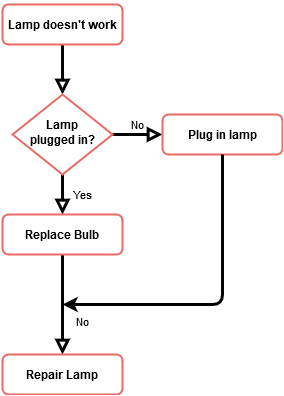
\includegraphics[height=6 cm, width=5cm]{images/Decision_control_3.png}
        	    % \caption{Caption}
        	    \label{fig:my_label}
        	\end{figure}
    \end{minipage}


\end{frame}

% \logo{
% 	\includegraphics[height=0.7cm]{images/logo_iai.jpg}
% 	\hspace{\dimexpr\paperwidth-2cm-5pt}
% 	\includegraphics[height=0.7cm]{images/logo_iai.jpg}
% 	}

\frame{\frametitle{Table of contents}
\tableofcontents\transdissolve
}
\AtBeginSection[]
  {
    \ifnum \value{framenumber}>1
      \begin{frame}<beamer>
      \frametitle{Plan}
      \tableofcontents[currentsection,currentsubsection]
      \end{frame}
    \else
    \fi
  }
% \AtBeginSection[currentsection, currentsubsection, hideothersubsection, sectionstyle=show/hide, subsectionstyle=show/shade] % Do nothing for \section*
% {\transblindshorizontal
% 	\begin{frame}<beamer>
% 		%\transdissolve
% 		\frametitle{currentsection}
% 		\tableofcontents[currentsection, hideothersubsections]%, pausesubsections]
% 	\end{frame}
% }

\section{Unit Outline}
    \begin{frame}{Unit-II Outline}
    
    \begin{block}{Completed in last class}
        \begin{itemize}
        \item Different syntax of if 
                    \begin{itemize}
                            \item  Sequential execution of C program
                             \item if block
                                \item if else block
                    \end{itemize}
        \end{itemize}
    \end{block}
       
    \begin{exampleblock}{To be continued in this class}
            \begin{itemize}
        \item Different syntax of if 
                    \begin{itemize}
                        \item Nested if else block
                        \item if else-if else block
                    \end{itemize}
        \end{itemize}
    \end{exampleblock}
          
            
    \end{frame}

\section{Different syntax of if }

    \subsection{Nested if else block}
    
    \begin{frame}{Recap Slide}
        \begin{minipage}{0.5\linewidth}
        \textbf{ Basic If syntax}
             \lstinputlisting[language=C]{code/basic-if-block-syntax.c}
        \end{minipage}%
        \begin{minipage}{0.5 \linewidth}
        \textbf{ Basic If-else syntax}
             \lstinputlisting[language=C]{code/if-else-syntax.c}
        \end{minipage}
    \end{frame}
    
    \begin{frame}{Recap slide-2 (if prog) }
             \lstinputlisting[language=C]{code/if-prog-2.c}
    \end{frame}
     \begin{frame}{Recap slide-3 (if-else prog)}
             \lstinputlisting[language=C]{code/if-else-prog-2.c}
       
    \end{frame}
    
    \begin{frame}{Nested if else}
    Inside if block or else block or both, if we again have :
    \begin{itemize}
        \item if block 
        \item or if-else block
    \end{itemize}
    it is called nested if-else block
    
    \textcolor{red}{Note} Show the Flowchart diagram on copy
    
    \end{frame}

    \begin{frame}{Nested if-else bock prog-1}
            \lstinputlisting[language=C]{code/nested-if-else-1.c}
        
    \end{frame}
    
    \subsection{ Use of Logical operator}
        \begin{frame}{Use of Logical operator}
         
            \begin{table}[]
    \centering
    \begin{tabular}{|c|c|c|} \hline
         \textbf{Symbol} & \textbf{Meaning} & \textbf{Examples} \\ \hline
        \multirow{4}{*}{\&\&}   & \multirow{4}{*}{AND} & (x \textgreater 5) \&\& (x \textless 10)        \\ 
         &          &  (y\textgreater 9)  \&\& (x \textless 40  \\ 
        &     & (marital\_status='M') \&\& (age \textgreater 30) \\ 
        &         & (BMI \textless 25) \&\& (height \textgreater 172)
        \\ \hline 
        
     \multirow{3}{*}{$||$}   & \multirow{3}{*}{OR}  & (total\_marks \textgreater 70) $||$ (quota =='S') \\
        &  & (sum \textgreater 40) $||$ (avg \textless20)    \\
        & & (data\_used \textgreater 1.5) $||$ (validity ==0) \\ \hline
       \multirow{3}{*}{!}   & \multirow{3}{*}{NOT} &  !(red\_zone)\\ 
       
       & & !(raining) \\ 
       & &  !(fever) \&\& !(cough) \\ \hline
       
    
    \end{tabular}
    
    \caption{Logical Operator Symbol, Meaning and examples}
                %\label{tab:my_label}
\end{table}
        
        \begin{itemize}
            \item Logical operator used to combine multiple statement into single expression
        \end{itemize}
   
        \end{frame}

\begin{frame}{Nested if-else bock prog-2 (Example 2.4)}
    \textbf{Exercise 2.4:}   The marks obtained by a student in 5 different subjects are input through the keyboard. The student gets a division as per the following rules:

    \begin{itemize}
        \item[-] Percentage above or equal to 60 - First division
        \item[-] Percentage between 50 and 59 - Second division
        \item[-] Percentage between 40 and 49 - Third division
        \item[-] Percentage less than 40 - Fail
    \end{itemize}
\end{frame}
    
\begin{frame}{Exercise-2.4 Method-1}
    
     \lstinputlisting[language=C,basicstyle=\scriptsize]{code/exercise-2.4-method-1.c} 
\end{frame}

\begin{frame}{Exercise-2.4 Method 1.1}
     \lstinputlisting[language=C, basicstyle=\scriptsize]{code/exercise-2.4-method-1.1.c} 
\end{frame} 

\begin{frame}{Exercise-2.4 Method 1.1}
    \begin{minipage}{0.6 \linewidth}
     \lstinputlisting[language=C, basicstyle=\scriptsize]{code/exercise-2.4-method-1.1.c} 
    \end{minipage}%
    \begin{minipage}{0.4 \linewidth}
     
     \textbf{Test case 1}
     \\Enter the marks in \%: 70 \\
        First division \\
    \textbf{Test case 2}
     \\Enter the marks in \%: 58 \\
       Second division  \\
    \textbf{Test case 3} 
     \\Enter the marks in \%: 35 \\
        Fail \\    
     \textbf{Test case 4} 
     \\Enter the marks in \%: 49 \\
        Third division \\     
    \end{minipage}
\end{frame}
 \begin{frame}{Points about Exercise 2.4 Method 1.1 solution}
    This program is build using nested if-else
    
 \end{frame}
\begin{frame}{Exercise-2.4 Method 2}
    
     \lstinputlisting[language=C, basicstyle=\scriptsize]{code/exercise-2.4-method-2.c} 
\end{frame} 
  
\end{document}
